\section{A linguagem do Wiring}[A linguagem do Wiring]

O Wiring é uma API (Application Programming Interface) (\autoref{wiringS}) da linguagem Processing, portando as funcionalidades de interface da linguagem, fazendo com que a programação do projeto seja independente da linguagem que o hardware entende, além também de ter todo o suporte gráfico que seu desenvolvimento (Processing) em Java o proporciona. 

\subsection{IDE}

O ambiente do Wiring (Integrated Development Environment ou IDE) possui um editor de texto e um compilador para escrever programas para o seu hardware. 

\begin{figure}[htb]
	\caption{\label{wiringIDE}Ambiente de Desenvovlimento do Wiring}
	\begin{center}
	    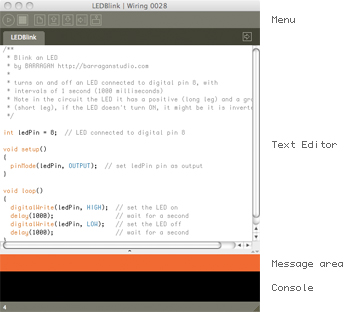
\includegraphics[scale=0.9]{artigo/refs/ide.jpeg}
	\end{center}
	%\legend{Fonte: Site da 3GPP}
\end{figure}

Nos próximos tópicos falaremos um pouco sobre os cabeçalhos e as principais funções que o Wiring nos proporcionou. Como este trabalho aborda o Wiring em relação ao Arduíno, iremos usar os cabeçalhos presentes no diretório de instalação do Arduíno.

\subsection{A biblioteca Wiring no Arduíno}

No diretório de instalação do Arduíno temos arquivos como wiring\_analog.c, wiring.c, wiring\_digital.c, wiring\_private.h  wiring\_pulse.c, wiring\_pulse.S, wiring\_shift.c e Arduino.h. Abaixo uma breve descrição de cada arquio

\begin{alineas}
    \item \textbf{Arduino.h}: Este cabeçalho possui todas as definições de constantes mais utilizadas como, HIGH, LOW, PI, EULER, definições de macros como  min(a,b), abs(x), lowByte, bitSet, e também protótipo das funções básicas como pinMode, digitalWrite, digitalRead. Também há definição de estruturas de dados como uint8\_t e bool .
    \item \textbf{wiring\_private.h}: Este cabeçalho possui mais definições de constantes e de macros muito utilizadas nas definições de função como cbi(sfr, bit) e sbi(sfr, bit). Aĺém disso há definições de constantes com base no microprocessador utilizado.
    \item \textbf{wiring.c}: Interface com as definições de funções como millis() e delay(). 
    \item \textbf{wiring\_analog.c} Interface com as definições de funções relacionadas aos pinos analógicos. Há funções como analogRead e analogWrite. 
    \item \textbf{wiring\_digital.c} Interface com as definições de funções relacionadas aos pinos digitais. Há funções como pinMode, digitalWrite e digitalRead.
    \item \textbf{wiring\_shift.c} Interface com as definições de funções relacionadas aos troca de determinado bit com base em um \emph{clock}. 
    \item \textbf{wiring\_pulse.c} Interface com as definições de funções relacionadas a pulsos com base em estado e tempo. 
    
    Abaixo um organograma com as dependências dos arquivos
    
    \begin{figure}[htb]
    	\caption{\label{wiringIDE}Organograma das funções citadas}
    	\begin{center}
    	    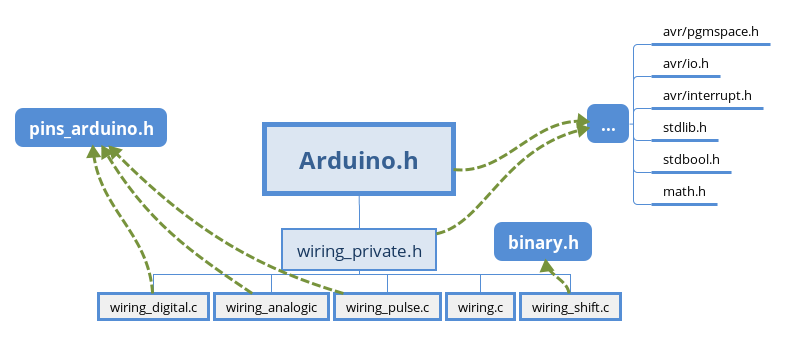
\includegraphics[scale=0.5]{artigo/refs/org_head_arduino}
    	\end{center}
    	\legend{Fonte: O autor}
    \end{figure}
    
\end{alineas}

\subsection{Principais Funções}

Quando iniciamos a aprendizagem do Arduino (ou outro hardware de prototipação) o \emph{Hello World}\footnote{Expressão utilizada quando escrevemos o primeiro programa em uma linguagem de programação} é fazer o led interno da placa piscar (\emph{blinking Led}). Este código inclusive, é o primeiro exemplo utilizado na tese de Barragán \cite[p.~39]{Barragan2004}. 

Com a instalação da IDE do Arduíno este código já vem pronto. As funções utilizadas no exemplo do Arduíno, além das principais setup() e loop(), são pinMode(), digitalWrite() e delay().\newline

\subsubsection{pinMode}

\definecolor{dkgreen}{rgb}{0,0.6,0}
\definecolor{gray}{rgb}{0.5,0.5,0.5}
\definecolor{mauve}{rgb}{0.58,0,0.82}
 
\lstset{
  language=C++,                
  basicstyle=\footnotesize,           
  numbers=left,                   
  numberstyle=\tiny\color{gray},  
  stepnumber=2,                             
  numbersep=5pt,                  
  backgroundcolor=\color{white},    
  showspaces=false,               
  showstringspaces=false,         
  showtabs=false,                 
  frame=single,                   
  rulecolor=\color{black},        
  tabsize=2,                      
  captionpos=b,                   
  breaklines=true,                
  breakatwhitespace=false,        
  title=\lstname,                               
  keywordstyle=\color{blue},          
  commentstyle=\color{dkgreen},       
  stringstyle=\color{mauve},     
}
\begin{lstlisting}
void pinMode(uint8_t pin, uint8_t mode)
{
uint8_t bit = digitalPinToBitMask(pin);
uint8_t port = digitalPinToPort(pin);
volatile uint8_t *reg, *out;

if (port == NOT_A_PIN) return;

// JWS: can I let the optimizer do this?
reg = portModeRegister(port);
out = portOutputRegister(port);

if (mode == INPUT) { 
	uint8_t oldSREG = SREG;
            cli();
	*reg &= ~bit;
	*out &= ~bit;
	SREG = oldSREG;
} else if (mode == INPUT_PULLUP) {
	uint8_t oldSREG = SREG;
            cli();
	*reg &= ~bit;
	*out |= bit;
	SREG = oldSREG;
} else {
	uint8_t oldSREG = SREG;
            cli();
	*reg |= bit;
	SREG = oldSREG;
}
}
\end{lstlisting}

\subsubsection{digitaWrite}

\begin{lstlisting}
void digitalWrite(uint8_t pin, uint8_t val)
{
	uint8_t timer = digitalPinToTimer(pin);
	uint8_t bit = digitalPinToBitMask(pin);
	uint8_t port = digitalPinToPort(pin);
	volatile uint8_t *out;

	if (port == NOT_A_PIN) return;

	// If the pin that support PWM output, we need to turn it off
	// before doing a digital write.
	if (timer != NOT_ON_TIMER) turnOffPWM(timer);

	out = portOutputRegister(port);

	uint8_t oldSREG = SREG;
	cli();

	if (val == LOW) {
		*out &= ~bit;
	} else {
		*out |= bit;
	}

	SREG = oldSREG;
}
\end{lstlisting}

\subsubsection{delay}

\begin{lstlisting}
void delay(unsigned long ms)
{
	uint32_t start = micros();

	while (ms > 0) {
		yield();
		while ( ms > 0 && (micros() - start) >= 1000) {
			ms--;
			start += 1000;
		}
	}
}
\end{lstlisting}